\chapter{\gls{DICOM}}

\section{What is DICOM?}
\begin{itemize}
\item \popup{Open}{Openly accessible and usable by anyone.}
  \popup{standard}{Actually is a set of standards.} created in 1992 by
  the \gls{ACR} and the \gls{NEMA} \cite{DICOM2025}.
\item It defines how to transfer (transport layers protocols:
  \gls{TCP} or \gls{UDP}), storage (filenames, structure of the
  filesystem, etc.), processing, display (such as \gls{GSDF}),
  perception, and use of information in medicine
  \cite{bushberg2011essential}, allowing devices and systems from
  different manufacturers to communicate and share medical image data
  seamlessly.
\end{itemize}.

\section{What is DICOM file?}
\begin{itemize}
\item \gls{DICOM} is a media container for medical signals
  (\gls{ECG} signals, \gls{PCG} audios, 2D images, 3D images, and videos).
\item A DICOM file, such as a single CT slice, consists of two
  distinct parts:
  \begin{enumerate}
  \item The \textbf{header} is a block of data that contains specific
    \popup{information}{Such as name, age, gender, date of birth, and
      technical data about the image (device used, resolution, codec,
      etc.).}  that complements the image
    (\popup{attributes}{Depending on the image and the circumstances,
      certain information is mandatory, while other attributes are
      optional.}), classified as
    \href{https://dicom.nema.org/medical/dicom/current/output/html/part06.html#PS3.6}{DICOM
      tags}.
  \item The \popup{\textbf{image} itself}{The signal in
      general.}. Notice that the metadata provided by \gls{DICOM} are
    different from the image's metadata.
  \end{enumerate}
\end{itemize}.

\section{Supported 1D-signals codecs}
\begin{itemize}
\item \gls{ECG} and \gls{PCG} signals are \popup{\gls{PCM}
    encoded}{Without any loss or data compression.} with up to 24
  bits/sample.
\end{itemize}

\section{Supported image codecs}
\begin{enumerate}
\item Lossless:
  \begin{enumerate}
  \item \popup{Raw}{As generated by the ADC (Analog Digital
      Converted.}
    \href{https://en.wikipedia.org/wiki/Endianness}{Little Endian}
    with up to 64 bits/grayscale-pixel
    (\href{https://en.wikipedia.org/wiki/Double-precision_floating-point_format}{double-precision
      floating-point format}).
  \item \gls{RLE}.
  \item \href{https://en.wikipedia.org/wiki/Lossless_JPEG}{JPEG Lossless}.
  \item \href{https://en.wikipedia.org/wiki/Lossless_JPEG\#JPEG_LS}{JPEG-LS}.
  \item \href{https://en.wikipedia.org/wiki/JPEG_2000}{JPEG 2000}
    (reversible path).
  \item \href{https://en.wikipedia.org/wiki/JPEG_XL}{JPEG XL}
    (reversible path).
  \item \href{https://en.wikipedia.org/wiki/Deflate}{Deflate}. Similar
    to \gls{PNG}.
  \end{enumerate}
\item Lossy:
  \begin{enumerate}
  \item \gls{JPEG}.
  \item \href{https://en.wikipedia.org/wiki/JPEG_2000}{JPEG 2000}
    (ireversible path).
  \item \href{https://en.wikipedia.org/wiki/JPEG_XL}{JPEG XL}
    (ireversible path).
  \end{enumerate}
\end{enumerate}

\section{Supported video codecs}
\begin{enumerate}
\item \gls{JPIP} (see Chapter~\ref{cha:JPEG2000}).
\item \gls{MPEG}-2 (see Chapter~\ref{cha:MPEG}).
\item \gls{HEVC} (see Chapter~\ref{cha:HEVC}).
\end{enumerate}

\section{Storage (example) (1/2)}
\begin{verbatim}
[USB Drive Root]          <- We are using an USB drive
+-- DICOMDIR              <- Binary File
+-- DICOM                 <- Folder
    +-- STUDY01           <- Folder
    |   +-- SERIES01      <- Folder
    |   |   +-- IMAG0001  <- Binary file
    |   |   +-- IMAG0002  <- Binary file
    |   |   +-- IMAG0003  <- Binary file
    |   |-- SERIES02      <- Folder
    |   |   |-- IMAG0004  :
    |   |   |-- IMAG0005
    +-- STUDY02
        +-- SERIES01
            +-- IMAG0006
            +-- IMAG0007
            +-- IMAG0008
\end{verbatim}

\section*{Storage (example) (2/2)}
Where the file \texttt{DICOMDIR} defines the content of the rest of the file system:
\begin{verbatim}
(0004,1130) DICOMDIR FILE
    (0004,1200) Patient Record: John Doe
        (0004,1200) Study Record: CT Brain 2025-09-02
            (0004,1200) Series Record: CT Scout
                (0004,1500) Image File Record: DICOM/STUDY01/SERIES01/IMAG0001
            (0004,1200) Series Record: CT Axial
                (0004,1500) Image File Record: DICOM/STUDY01/SERIES02/IMAG0002
                (0004,1500) Image File Record: DICOM/STUDY01/SERIES02/IMAG0003
            :
\end{verbatim}

\section{Transmission using the \gls{ULP}}
\begin{itemize}
\item A pair of \gls{DICOM} devices communicate using a client-server
  model based on the \popup{DICOM \gls{ULP}}{An application-layer
    protocol.} which runs on top of standard TCP/IP.
\item Steps:
  \begin{enumerate}
  \item \textbf{Association establishment (handshake)}: the
    application entities agree about the \popup{task to be
      performed}{For example, sending an image.}, and the
    \popup{transfer syntax}{The compression method (e.g., JPEG, RLE)
      and byte order that will be used for the data.}.
  \item \textbf{Data Exchange (conversation)}: The sender sends the
    image using a C-STORE-RQ (Request) message (which the DICOM image,
    including the DICOM header) and, if the message has been
    successfully, the receiver send a C-STORE-RSP (Response).
  \item \textbf{Association Release (Hanging Up)}: After all data has
    been successfully sent and acknowledged, the devices terminate the
    association.
  \end{enumerate}
\end{itemize}

\section{Display (brightness) standarization (1/2)}
\begin{itemize}
\item To ensure \emph{visual consistency}, that image looks the same
  regardless of which monitor or display device it's viewed on.
\item This is achieved through the \gls{GSDF}, that expresses the
  \popup{luminance}{Luminosity, usually measures in candelas per
    square meter (cd/m2).} that a display should produce as a function
  of the pixels values. Thus, the luminance that a pixel with with
  \popup{value}{P-Value in terms of the standard notation.} $x$ (the
  should have is
  \begin{equation}
    L(j) = \exp\left(\sum_{i=0}^{9}a_i\big(\ln j(x)\big)^i\right),
  \end{equation}
  where
  \begin{center}
  \begin{tabular}{l}
    $a_0 = -1.3011877$, \\
    $a_1 = -2.5840191E-2$, \\
    $a_2 = 8.0242636E-2$, \\
    $a_3 = -1.0320229E-1$, \\
    $a_4 = 1.3646699E-1$, \\
  \end{tabular}
  \begin{tabular}{l}
    $a_5 = 2.8745620E-2$, \\
    $a_6 = -2.5468404E-2$,\\
    $a_7 = -3.1978977E-3$, \\
    $a_8 = 1.2992634E-4$, \\
    $a_9 = 1.3635334E-3$,
  \end{tabular}
  \end{center}
  and where
  \begin{equation}
    j(x) = j_{\text{min}} + \frac{j_{\text{max}} - j_{\text{min}}}{n(x)},
  \end{equation}
  being $j_{\text{min}}$ and $j_{\text{max}}$ are the \popup{minimum
    and maximum \gls{JND} index within the luminance range of the
    display}{That a normal human being can recognize in the display
    which is being standardized.}, and where
  \begin{equation}
    n(x) = \frac{x}{2^N-1},
  \end{equation}
  where $N$ is thee number of bits/pixel.
\end{itemize}
\begin{center}
  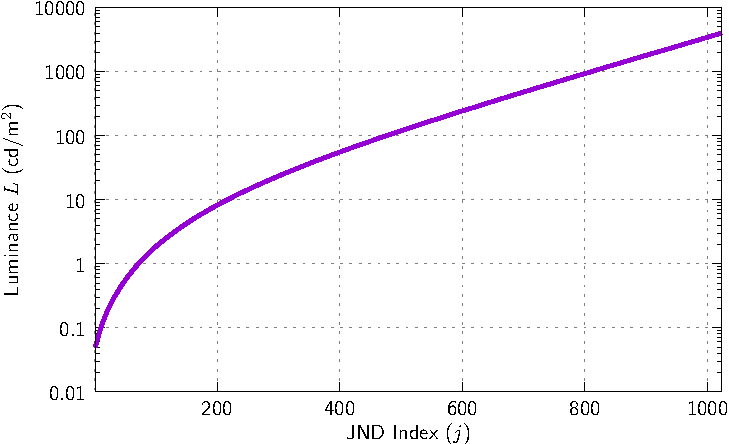
\includegraphics[width=0.7\textwidth]{GSDF}
\end{center}

\section*{Display standarization (2/2)}
\begin{itemize}
\item This way, equal steps in pixel values correspond to equal
  perceptual differences (\glspl{JND}), in other words, a
  \popup{step}{An increment in one in the integer value of ...} in
  \gls{JND} corresponds as the smallest brightness change detectable
  by the average human eye.
\end{itemize}
